\ifdefined\activerhandout 
\documentclass[12pt,aspectratio=1610,handout]{beamer}
\else
\documentclass[12pt,aspectratio=1610]{beamer}
\fi

%\usepackage[french]{babel} %=> erreur avec les tikz du moteur
\usepackage[T1]{fontenc}
\usepackage[utf8]{inputenc}
\usepackage{lmodern}
\usepackage{hyperref}
\usepackage{smartdiagram}
\usepackage{tikz}
\usepackage{animate}
\usepackage{tikzpeople}
\usepackage{appendixnumberbeamer}
\usepackage[labelformat=empty]{caption}
%\usepackage{pictochrono}
\usepackage{fontawesome5}
\usepackage{awesomebox}

\usetheme{Warsaw}
\setbeamertemplate{page number in head/foot}[totalframenumber]

\newcommand{\anglais}[1]{(\textit{\color{blue}#1})}
\newcommand{\legende}[2]{\caption[#1 (Source : \cite{#2})]{#1}}
\newcommand{\histoire}[1]{\begin{awesomeblock}{2pt}{\faBook}{black!75}#1\end{awesomeblock}}
\newcommand{\info}[1]{\begin{awesomeblock}{2pt}{\faInfoCircle}{black!75}#1\end{awesomeblock}}
\newcommand{\question}[1]{\begin{awesomeblock}{2pt}{\faQuestionCircle}{black!75}#1\end{awesomeblock}}
\newcommand{\alerte}[1]{\begin{awesomeblock}{2pt}{\faExclamationCircle}{black!75}#1\end{awesomeblock}}
\newcommand{\astuce}[1]{\begin{awesomeblock}{2pt}{\faLightbulb}{black!75}#1\end{awesomeblock}}
\newcommand{\exemple}[1]{\begin{awesomeblock}{2pt}{\faSearch}{black!75}#1\end{awesomeblock}}
\newcommand{\definitionAConnaitre}[1]{\begin{awesomeblock}{2pt}{\faCog}{black!75}#1\end{awesomeblock}}

\newcommand{\qmcBia}[7]{
%1 : titre slide
%2 : numéro de la bonne réponse
%3 : Inititulé de la question
%4, 5, 6, et 7 : propositions de réponse
\begin{frame}{#1}
\begin{awesomeblock}{2pt}{\faQuestion}{black!75}
#3
	\begin{enumerate}
	\ifnum#2=1
		\only<1>{\item #4}
		\only<2>{\item \textbf{#4}}
	\else
		\item #4
	\fi
	\ifnum#2=2
		\only<1>{\item #5}
		\only<2>{\item \textbf{#5}}
	\else
		\item #5
	\fi
	\ifnum#2=3
		\only<1>{\item #6}
		\only<2>{\item \textbf{#6}}
	\else
		\item #6
	\fi
	\ifnum#2=4
		\only<1>{\item #7}
		\only<2>{\item \textbf{#7}}
	\else
		\item #7
	\fi
	\end{enumerate}
	\pause
\end{awesomeblock}
\end{frame}
}

\subtitle{BIA - Brevet d'Initiation Aéronautique}
\author{Clément \textsc{Vermot-Desroches}}
\institute{Collège Aliénor d'Aquitaine\\Martignas-sur-Jalle}
\date{\today}

%\AtBeginSection[]
%{
%    \begin{frame}
%        %\frametitle{Table of Contents}
%        \tableofcontents[currentsection]
%    \end{frame}
%}

\AtBeginSubsection[]
{
    \begin{frame}
        %\frametitle{Table of Contents}
        \tableofcontents[currentsection,currentsubsection]
    \end{frame}
}

\title[Séance 3 - Hélices et Réacteurs]{Séance 3 \\ Hélices \& Turbomoteurs}

\begin{document}
 \begin{frame}
 \titlepage
 \end{frame}
 
 \begin{frame}
 \tableofcontents
 \end{frame}
 
 \section{Hélices}
	\begin{frame}{Question}
	
	\question{A quoi servent les hélices ?}
	
	\pause
	
	\question{Quelles sont les caractéristiques d'une hélice ?}
	
	\end{frame}	
	
	\begin{frame}{Historique}
	L'hélice fut le premier dispositif crée pour transmettre la puissance des moteurs.
	\end{frame}	 
 
 
 
 
 \section{Turbomoteurs}
 \subsection{Réacteurs}
 \begin{frame}{Turboréacteur simple flux}
 	\begin{figure}[H]
  		\centering
    		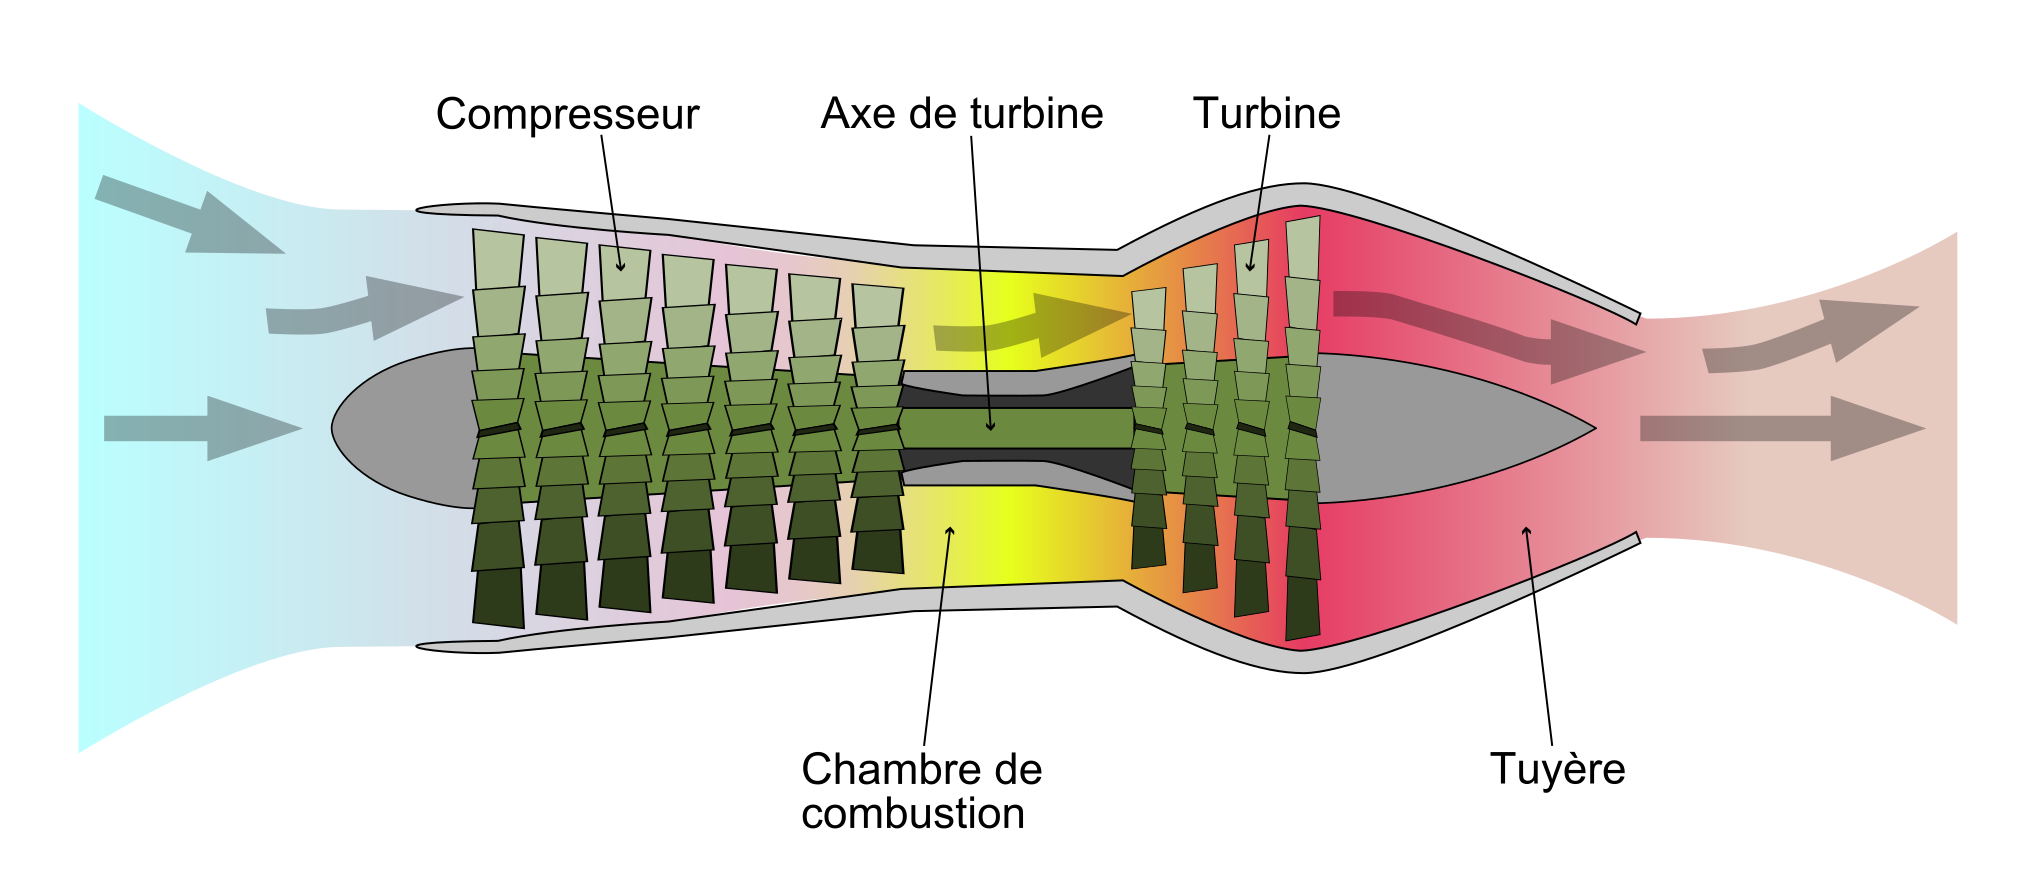
\includegraphics[width=1.0\textwidth]{01-EtudeAeronefs/img/turbomachines/turboreacteur-simpleFlux.pdf}
  		\legende{Schéma d'un turboréacteurs simple flux}{img:turboreacteur-simpleFlux}
	\end{figure}	
  \end{frame}
  \begin{frame}{Turboréacteur double flux}
	\begin{figure}[H]
  		\centering
    		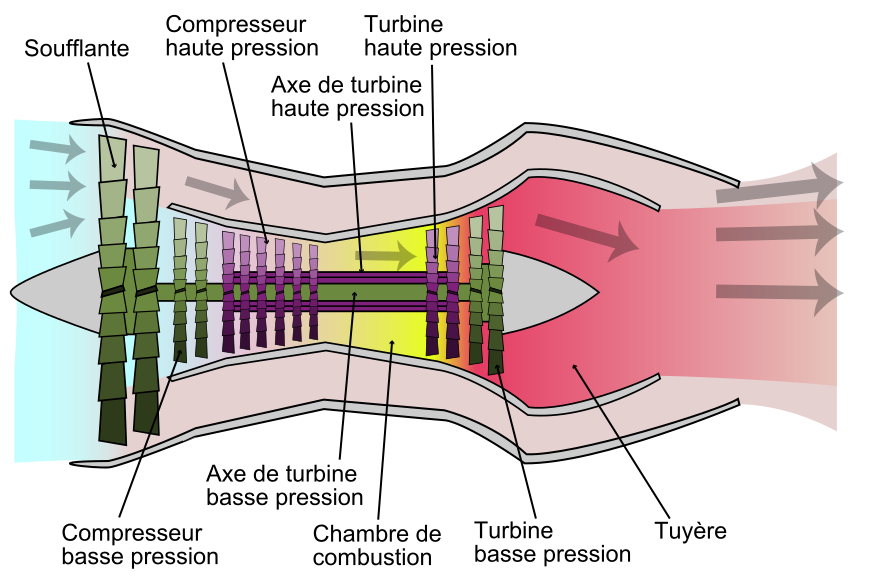
\includegraphics[width=0.6\textwidth]{01-EtudeAeronefs/img/turbomachines/turboreacteur-doubeFlux.pdf}
  		\legende{Schéma d'un turboréacteurs double flux}{img:turboreacteur-doubeFlux}
		\end{figure}	
 \end{frame}
 \subsection{Turbopropulseurs}
 
   \begin{frame}{Turbopropulseur}
	\begin{figure}[H]
  	\centering
    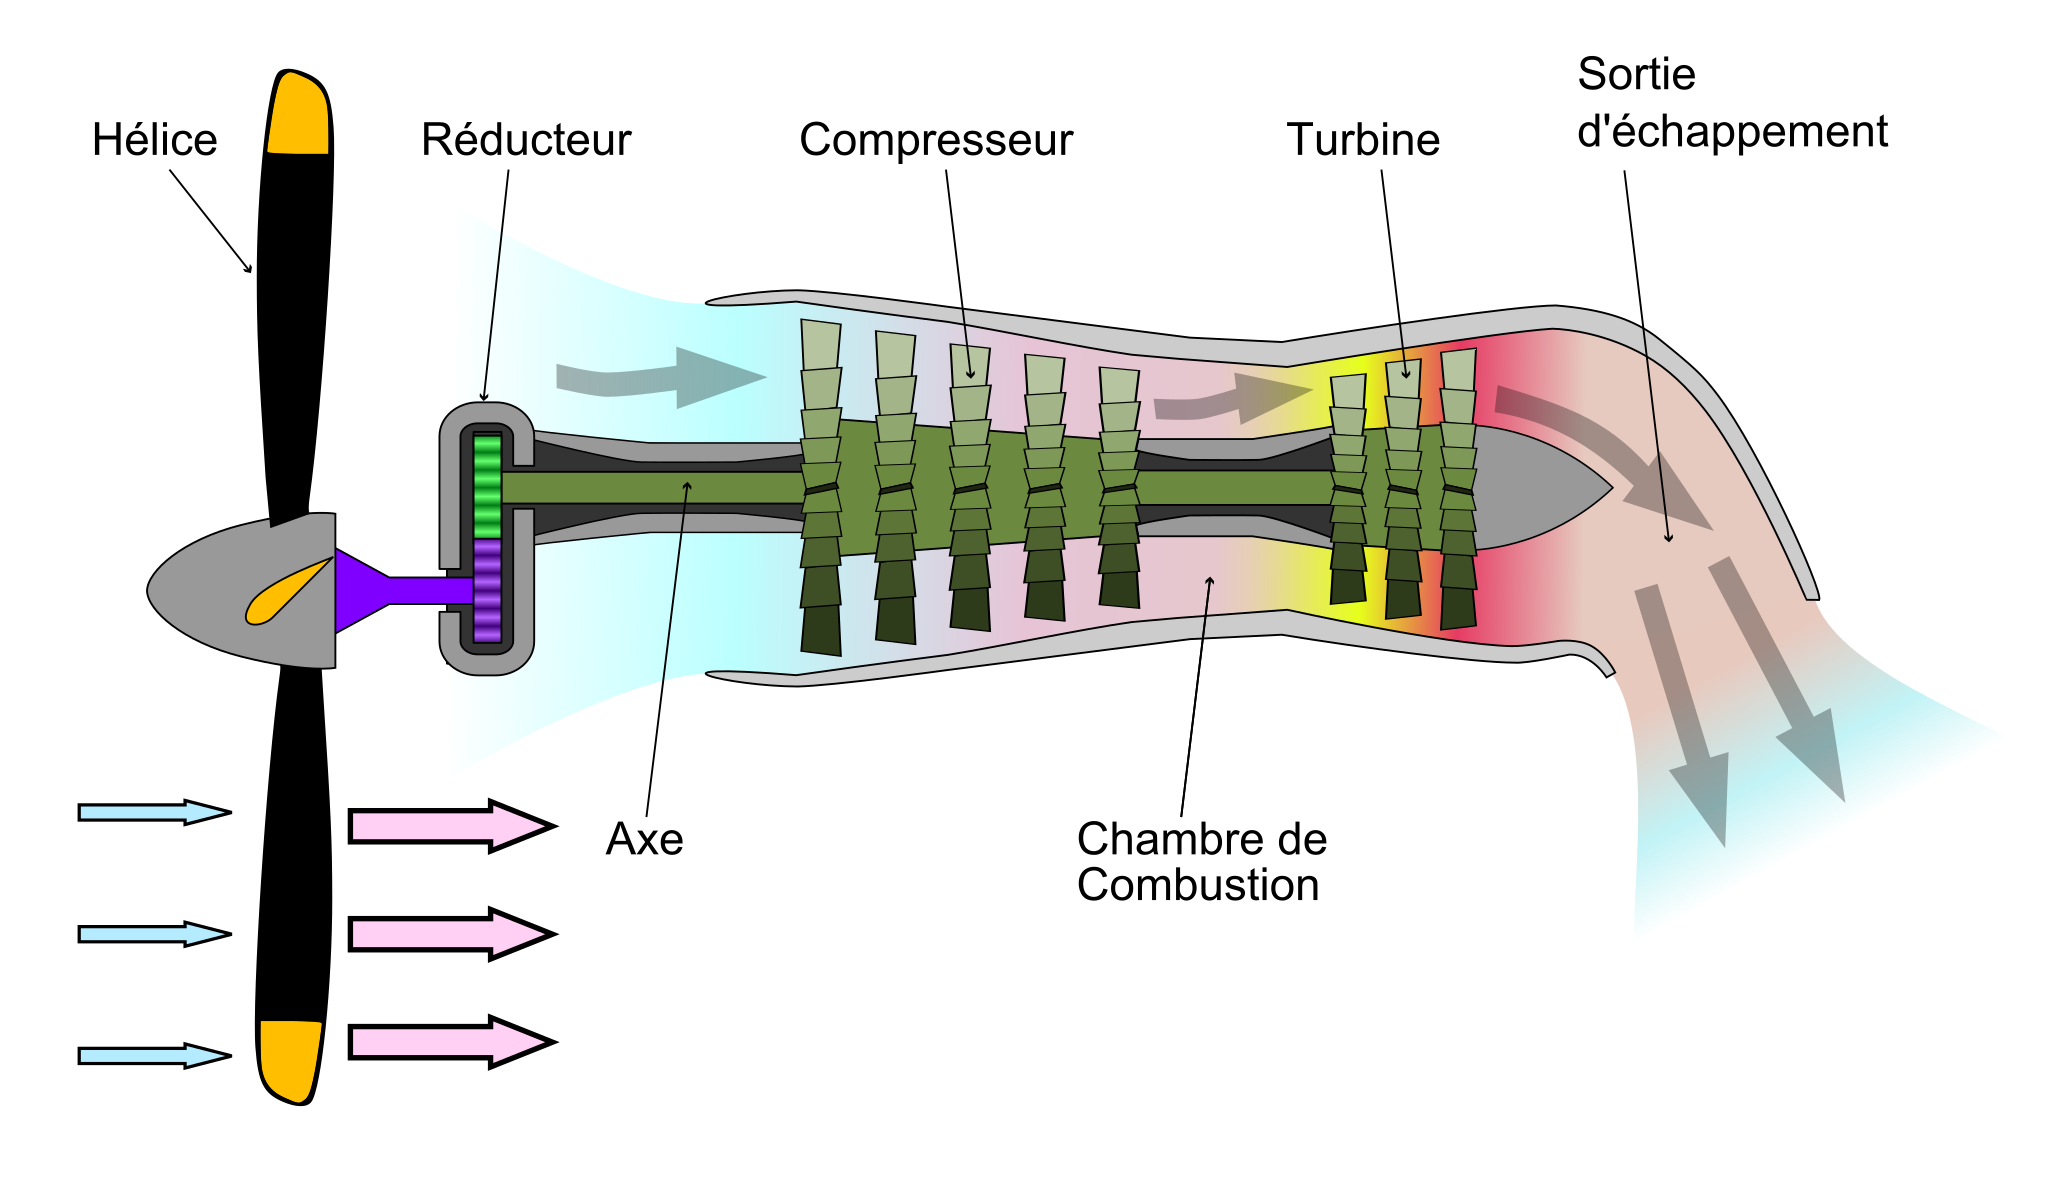
\includegraphics[width=0.75\textwidth]{01-EtudeAeronefs/img/turbomachines/turbopropulseur.pdf}
  	\legende{Schéma d'un turbopropulseur}{img:turbopropulseur}
	\end{figure}	
 \end{frame}
 
\appendix 
\section{QCM}
%\qmcBia{Étude des aéronefs}
%{3}{\begin{figure}[H]
%  		\centering
%    		\includegraphics[width=0.2\textwidth]{01-EtudeAeronefs/img/PWWasp.jpg}
%	\end{figure}	
%	La disposition des cylindres de ce moteur est :}
%{en ligne}
%{en V}
%{en étoile}
%{à plat} 


\qmcBia{Étude des aéronefs}
{4}{Un turbopropulseur}
{est un pulsoréacteur précédé d'un réducteur et d'une hélice}
{est un statoréacteur précédé d'un réducteur et d'une hélice}
{est un moteur à pistons équipé d'un turbocompresseur}
{est un turboréacteur précédé d'un réducteur et d'une hélice} 
 
\ifdefined\activerbibliobeamer
\begin{frame}[allowframebreaks]
\frametitle{Bibliographie}
\printbibliography
%\nocite{*}
\end{frame}
\fi 
 
\end{document}
